\scanpage{406}
\mspage{504}
ly take $f=1$, and we will have
\[
\alpha=\underline u,\qquad\text{whence}\qquad\underline a=1,
\]
on the other hand, let us note that $\mu\in\{\pm1\}\inserted{\text{i.e. }\mu}=(-1)^k$ $(k\in\mathbb Z/2\mathbb Z)$, we will have $\varepsilon=\varepsilon'=\mu$, and if $\mu=1$ \inserted{(i.e. $u\in\mathrm{Sl}(2,\mathbb Z)$)} we will have $\beta=\underline u$ (\deleted{since} hence $\underline b=1$, otherwise $\beta=\deleted{\unsure{\tau_\infty}}u\tau_\infty$ hence $\underline b=\tau_\infty$), in all cases we will have
\[
\beta=u\tau_\infty^k,\qquad\underline b=\tau_\infty^k,
\]
in summary
\[
\tag{37}
\begin{gathered}
\underline u=\left(
\underset{\substack{\rotatebox{90}{$\in$}\\\Gamma B'_0}}{\underline u=u},
\underset{\substack{\rotatebox{90}{$\in$}\\\Gamma T_\rho}}{\underline a=1},
\underset{\substack{\rotatebox{90}{$\in$}\\\Gamma N'_\sigma}}{\underline b=\tau_\infty^k}
\right)
\in
\underset{\substack{\rotatebox{90}{$=$}\\\inserted{\mathcal M_{\rho,\sigma}[0](\widehat{\mathbb Z})}}}
{\deleted{\unsure{\mathcal M}}\,\unsure{S\mathcal G|\mathcal G}_{\rho,\sigma}^{*}(\unsure{0})(\widehat{\mathbb Z})}
\subset\left(B'_0\times T_\rho\times N'_\sigma\right)(\widehat{\mathbb Z}).
\end{gathered}
\]

\deleted{$2^\circ)$ $r_1=-\tau'_0=\begin{pmatrix}-1&1\\0&1\end{pmatrix}$. To it we can \unsure{apply the}}

But this is not an element in \deleted{\unsure{preceding paragraph|preceding argument}} \unsure{normalized} form --- \deleted{besides \unsure{we}} \inserted{i.e.} it is not in $\Gamma\mathcal G_{\rho,\sigma}^{*}(0)$, unless $\lambda=0$. \deleted{\unsure{We will have}}

$2^\circ)$ $r_1=-\tau'_0=\begin{pmatrix}-1&1\\0&1\end{pmatrix}$, this is precisely a case that falls under \unsure{the preceding remarks}, we will have
\[
\tag{38}
\unsure{r_1|\tau_1}=-\tau'_0=
\left(\underline u_1=-\tau'_0=\begin{pmatrix}-1&1\\0&1\end{pmatrix},\ \underline a=1,\ \underline b=\tau_\infty\right)
\in\mathcal M_{\rho,\sigma}[0](\mathbb Z)
\]
\margin{\uline{N.B.} \unsure{reducing} modulo $L_0\subset\widetilde G_{\rho,\sigma}^{+}$, $\tau_\infty$ and $r_1$ have the same image in $\tau_{\rho,\sigma}$, namely $(-1,1,\tau_\infty)$.}

$3^\circ)$ $r_0=\tau'_\infty=\begin{pmatrix}0&1\\1&0\end{pmatrix}$, this time we have an automorphism \inserted{of $\widetilde G_{0,3}^{+}$ \unsure{or} $\widetilde G_{0,3}^{+\wedge}$} which does not normalize $L_0$ --- that is better, if we want $r_0,r_1,r_\infty$ to generate $\mathrm{Gl}(2,\mathbb Z)$ (or even ``only'' $\mathrm{Gl}(2,\mathbb Z)'$) !

We have $\tau'_\infty=\tau_\infty\sigma_\infty$, so its image in $\mathcal M_{\rho,\sigma}(\mathbb Z)\subset\mathcal M_{\rho,\sigma}(\widehat{\mathbb Z})$ is \deleted{\unsure{like}} the product of the images of $\tau_\infty$ and $\sigma_\infty$ --- the first was computed in $1^\circ$, the second is tautological since $SG\simeq\widetilde G_{\rho,\sigma}^{+}$ and $\sigma_\infty\in SG(\mathbb Z)$. We will note that \deleted{$\unsure{\tau'_\infty}$} $r_0=\tau'_\infty$ thus has the same image
\margin{405}

\scanpage{407}
\mspage{\unsure{504}}

in $\tau_{\rho,\sigma}(\mathbb Z)$ as $r_\infty=\tau_\infty$ and $r_1=-\tau'_0$, it is always the same element \deleted{\illegible{1}}
\[
(39)\qquad (-1,1,\tau_\infty)\in
\left(\underset{\substack{\wr\\\mathbb G_m}}{T_0}\times T_\rho\times N'_\sigma\right)(\mathbb Z)
\]

Let us moreover compute
\[
T_0\times T_\rho\times N'_\sigma(\mathbb Z)
=T_0(\mathbb Z)\times T_\rho(\mathbb Z)\times N'_\sigma(\mathbb Z)
\]
We have
\[
(40)\quad
\left\{
\begin{array}{ll}
T_0\simeq\mathbb G_m,\quad T_0(\mathbb Z)\simeq\{\pm1\}&\\[2pt]
T_\rho(\mathbb Z)\simeq(\mathbb Z+\mathbb Z.\rho)^*\simeq\mathbb Z/6\mathbb Z
&\begin{array}{l}\text{group generated}\\\text{by }\rho\end{array}\\[2pt]
N'_\sigma(\mathbb Z)\simeq\{1,\tau_\infty\}.T_\sigma(\mathbb Z)
&\text{(semidirect product)}\\[2pt]
T_\sigma(\mathbb Z)\simeq(\mathbb Z+\mathbb Z\sigma)^*\simeq\mathbb Z/4\mathbb Z
&\begin{array}{l}\text{group generated}\\\text{by }\sigma\end{array}\\[2pt]
N'_\sigma(\mathbb Z)\simeq D_4
&\begin{array}{l}\text{\unsure{dihedral} group of order \unsure{4}}\\\text{(``symmetries of the square'')}\end{array}
\end{array}
\right.
\]
whence
\[
(41)\quad (T_0\times T_\rho\times N'_\sigma)(\mathbb Z)
\simeq
\underbrace{(\mathbb Z/2\mathbb Z)}_{\substack{\text{\unsure{group generated}}\\\text{by }\tau_\infty}}
.\,(\mathbb Z/2\mathbb Z\times\mathbb Z/6\mathbb Z\times\mathbb Z/4\mathbb Z)
\]
\hfill $\tau_\infty$ operates \unsure{trivially} on the first two factors and by symmetry on the last
\[
\simeq\underbrace{\mathbb Z/2\mathbb Z\times\mathbb Z/6\mathbb Z\times
\underbrace{(\mathbb Z/2\mathbb Z.\mathbb Z/4\mathbb Z)}_{D_4}}_{\unsure{\downarrow}}
\]

On the other hand
\margin{\uline{N.B.} the condition $\det\underline a=\varepsilon'\det\underline u$, $\varepsilon'^2=1$ is automatic, since $\mathbb G_m(\mathbb Z)=\{\pm1\}$.}
\[
\begin{aligned}
(42)\quad S\mathcal G^*_{\rho,\sigma}(0)(\mathbb Z)
&=\tau_{\rho,\sigma}\deleted{\unsure{[0]}}(\mathbb Z)
=\left\{\underbrace{(u,a,b)}_{\in T_0\times T_\rho\times N'_\sigma(\mathbb Z)}\mid\det u=\det b\right\}\\
&\simeq\deleted{D_4}(T_\rho\times N'_\sigma)(\mathbb Z)\simeq\mathbb Z/6\mathbb Z\times D_4
\end{aligned}
\]
\deleted{and \unsure{arrow specified by}}
\deleted{\diagram{\begin{tikzcd}[ampersand replacement=\&,column sep=large]
\underset{\substack{\Vert\\\{\tau_\infty^i\sigma^j\mid i\in\mathbb Z/2\mathbb Z,\ j\in\mathbb Z/4\mathbb Z\}}}{D_4}
\arrow[r]\&\unsure{\mathcal M}_{\rho,\sigma}[0](\mathbb Z)
\end{tikzcd}}}
\deleted{$\tau_\infty,$}
\margin{406}

\scanpage{408}
\mspage{505}

the remarkable element, common image of $r_0=\tau'_\infty$, $r_1=-\tau'_0$, $r_\infty=\tau_\infty$ corresponds to the element $(1,\tau_\infty)$ of $\mathbb Z/6\mathbb Z\times(D_4\simeq\{1,\tau_\infty\}.\mathbb Z/4\mathbb Z)$.

This also gives us an expression for \deleted{$\mathcal M_{\rho,\sigma}(\mathbb Z)$, \unsure{hence}}
\[
(43)\qquad
\left\{
\begin{array}{l}
\mathcal M_{\rho,\sigma}(\mathbb Z)\simeq
\underset{\mathcal M_{\rho,\sigma}(0)(\mathbb Z)}{\underline{\tau_{\rho,\sigma}(\mathbb Z)}}
.\,\mathrm{Sl}(2,\mathbb Z)\\[5pt]
\hspace{4em}\text{(semidirect product)}\\[5pt]
\hspace{4em}\simeq(\mathbb Z/4\mathbb Z\times D_4).\,\mathrm{Sl}(2,\mathbb Z)
\end{array}\right.
\]
where $\mathbb Z/4\mathbb Z\times D_4$ operates on $\mathrm{Sl}(2,\mathbb Z)$ via the composite canonical homomorphism

\noindent$(44)$\quad
\diagram{\begin{tikzcd}[ampersand replacement=\&,column sep=large]
\mathbb Z/4\mathbb Z\times D_4
\arrow[r,"{\substack{\text{canonical}\\\text{projection}}}"']
\&D_4\arrow[r,"{\text{homomorphism}}","{\text{canonical}}"']\&\{1,\tau_\infty\}
\end{tikzcd}}

$\tau_\infty$ operating on $\mathrm{Sl}(2,\mathbb Z)$ by \unsure{inner automorphism} with the matrix
\[
\tau_\infty=\begin{pmatrix}-1&0\\0&1\end{pmatrix}.
\]
\margin{!}

We note that the canonical \unsure{epimorphism}
\diagram{\begin{tikzcd}[ampersand replacement=\&]
\mathcal M_{\rho,\sigma}\arrow[r]\&\mu_2\times\mu_2
\end{tikzcd}}
\unsure{\deleted{factors}} through \unsure{homomorphism} $\tau_{\rho,\sigma}$, and induces homomorphisms on the integral points

\noindent$(45)$\quad
\diagram{\begin{tikzcd}[ampersand replacement=\&,column sep=small]
\mathcal M_{\rho,\sigma}(\mathbb Z)\arrow[r]
\&\tau_{\rho,\sigma}(\mathbb Z)\simeq\mathbb Z/\deleted{\unsure{4}}\inserted{6}\mathbb Z\times D_4\arrow[r]
\&\begin{array}{c}(\mu_2\times\mu_2)(\mathbb Z)\\\simeq\{\pm1\}\times\{\pm1\}\end{array}
\end{tikzcd}}

This homomorphism is zero on $\mathbb Z/6\mathbb Z\times\underbrace{\mathbb Z/4\mathbb Z}_{D_4^+}$ \deleted{$\unsure{\det a}$} (corresponds to determinants equal to $1$), and on $\tau_\infty$ takes the value $(-1,-1)$. We \unsure{will note} therefore that this homomorphism on the integral points is
\margin{407}

\scanpage{409}

not surjective.

\uline{Center of $\mathcal M_{\rho,\sigma}$}$=\mathcal M_{\rho,\sigma}(0).\,SG$. It is the \deleted{semi-}direct product \unsure{of the the} subgroup of the center of $\mathcal M_{\rho,\sigma}(0)$ which operates \unsure{trivially} on $SG$, by the \inserted{subgroup of the \unsure{points} \deleted{\unsure{fixed}}\inserted{\unsure{invariant}} under $\mathcal M_{\rho,\sigma}$} center of $SG$. The latter \inserted{center} is well known, it is $\mu_2$, \deleted{It \unsure{is the same}} \inserted{and $\mathcal M_{\rho,\sigma}$ operates on it \unsure{trivially}.}

\margin{\uuline{false}, an element $g.f$ of a $1/2$ direct product can be central without $g$ operating \unsure{trivially} on the \unsure{invariant} group $\unsure{G}$.}
\figure{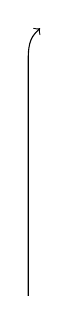
\begin{tikzpicture}[x=0.25cm,y=0.25cm]
\draw[->] (0,0)--(0,12).. controls (0,13) and (0.2,13.2)..(0.6,13.6);
\end{tikzpicture}}

On the other hand the subgroup of
\[
\mathcal M_{\rho,\sigma}(0)\simeq\tau_{\rho,\sigma}\subset B'_0\times T_\rho\times N'_\sigma
\]
which operates trivially on $SG$, is \inserted{the intersection of $\tau_{\rho,\sigma}$ with} $(\deleted{\unsure{\mu_2}}\inserted{1}\times T_\rho\times N'_\sigma)$, for $B'_0$ operates \unsure{trivially} \deleted{$\mu_2\unsure{\subset}B'_0$} (since
\[
(46)\qquad B'_0\cap\underbrace{\mu_2}_{\substack{\text{center of}\\SG}}=\{1\}
\]
. It is therefore the subgroup of the
\[
(47)\qquad
\left\{\left(1,\underset{\in\,\Gamma T_\rho}{\underline a},\underset{\in\,\Gamma N'_\sigma}{\underline b}\right)\mid(\det\underline a)^2=1,\ \det\underline b=1\right\}
\]

\margin{\unsure{no!}}
\uline{Remains} : determine \uline{the center of} $\tau_{\rho,\sigma}$, extension of $\mu_2\times\mu_2$ by $\tau^0_{\rho,\sigma}\simeq\mathcal G^*_{\rho,\sigma}(0)^0\subset T_0^0\times T_\rho\times\deleted{\unsure{N'_\sigma}}\inserted{T_\sigma}$. Since $\tau^0_{\rho,\sigma}$ is commutative, it suffices to determine the action of $\mu_2\times\mu_2$ on $\tau^0_{\rho,\sigma}$, and to determine its subgroup of invariants.
\margin{This will give at least the intersection of the center \unsure{with} $\tau^0_{\rho,\sigma}$.}
\margin{408}

\scanpage{410}
\mspage{506}

Let us note that we have
\[
\tau_{\rho,\sigma}=S\mathcal G^*_{\rho,\sigma}(0)\subset\mathcal G^*_{\rho,\sigma}(0)\simeq T_0\times T_\rho\times N'_\sigma
\]
and we have a homomorphism of exact sequences

\noindent$(48)$\quad
\diagram{\begin{tikzcd}[ampersand replacement=\&,column sep=large,row sep=large]
1\arrow[r]\&\tau^0_{\rho,\sigma}\arrow[r]\arrow[d,hook]
\&\tau_{\rho,\sigma}\arrow[r,"{(\underline u,\underline a,\underline b)\mapsto(\varepsilon(\underline b),\det\underline a/\det(\underline u))}"]\arrow[d,hook]
\&\mu_2\times\mu_2\arrow[r]\arrow[d,"{\substack{\text{first}\\\text{projection}}}"]\&1\\
1\arrow[r]\&\unsure{T_0}\times T_\rho\times\deleted{\unsure{N'_\sigma}}\inserted{T_\sigma}\arrow[r]
\&T_0\times T_\rho\times N'_\sigma\arrow[r]\&\mu_2\arrow[r]\&1
\end{tikzcd}},

which shows that the action of $\mu_2\times\mu_2$ on \deleted{$\unsure{\tau}$} $\tau^0_{\rho,\sigma}$ takes place through the projection of $\mu_2\times\mu_2$ onto its first factor, and this by the operation of the latter on $T_0\times T_\rho\times T_\sigma$ which operates trivially on $T_0\times T_\rho$, and which on $T_\sigma$ is the canonical operation of $\mu_2$ on $T_\sigma$, $\sigma\mapsto\varepsilon\sigma$, whose invariants are reduced to the scalars $\mathbb G_m$. \deleted{Thus we find} \inserted{This reasoning} shows, more generally, that the \unsure{trace} \inserted{of the center of $\tau_{\rho,\sigma}$} on the subgroup $\tau'_{\rho,\sigma}\subset\tau_{\rho,\sigma}$ kernel of

\diagram{\begin{tikzcd}[ampersand replacement=\&,column sep=large]
\tau_{\rho,\sigma}\arrow[r]\&\mu_2\times\mu_2\arrow[r,"{\text{1\textsuperscript{st} projection}}"]\&\mu_2\\
(\underline u,\underline a,\underline b)\arrow[rr,mapsto]\&\&\varepsilon(\underline b)
\end{tikzcd}}

is also the trace, on this subgroup, of $T_0\times T_\rho\times\mathbb G_m$. Moreover, since $\mu_2$ operates \uline{faithfully} on $T_\sigma$ via $\sigma\mapsto\varepsilon\sigma$, we see \deleted{that} at once that it also operates faithfully on $\tau'_{\rho,\sigma}$ (which indeed maps \uline{\unsure{epimorphically}} onto $T_\sigma$ !) so we have

\diagram{\begin{tikzcd}[ampersand replacement=\&,column sep=large]
\uline{\mathrm{Centre}}(\tau_{\rho,\sigma})\subset\tau'_{\rho,\sigma}=\operatorname{Ker}\bigl(\tau_{\rho,\sigma}
\arrow[r,"{(\underline u,\underline a,\underline b)\mapsto\varepsilon(\underline b)}"]\&\mu_2\bigr)
\end{tikzcd}}
\margin{409}